\documentclass[12pt,a4paper,oneside]{book}
\usepackage[utf8]{inputenc}
\usepackage[T1]{fontenc}
\usepackage[a4paper,top=3cm,bottom=2cm,left=3cm,right=3cm,marginparwidth=1.75cm]{geometry}
\usepackage[spanish]{babel}
\usepackage{times}
\usepackage{graphicx}
\usepackage{amssymb,amsmath}
\usepackage{tikz}
\usetikzlibrary{shapes,arrows,spy,positioning,snakes}
\newcommand{\R}{\mathbb{R}}
\newcommand{\N}{\mathbb{N}}
\newcommand{\Z}{\mathbb{Z}}
\newcommand{\C}{\mathbb{C}}
\usepackage{textcomp}
\usepackage{ragged2e}

\usepackage{tikz,pgfplots}

\usepackage{listings}
\usepackage{xcolor}

\definecolor{codegreen}{rgb}{0,0.6,0}
\definecolor{codegray}{rgb}{0.5,0.5,0.5}
\definecolor{codepurple}{rgb}{0.58,0,0.82}
\definecolor{backcolour}{rgb}{0.95,0.95,0.92}

\lstdefinestyle{mystyle}{
	backgroundcolor=\color{backcolour},   
	commentstyle=\color{codegreen},
	keywordstyle=\color{magenta},
	%numberstyle=\tiny\color{codegray},
	stringstyle=\color{codepurple},
	basicstyle=\ttfamily\footnotesize,
	breakatwhitespace=false,         
	breaklines=true,                 
	captionpos=b,                    
	keepspaces=true,                 
	numbers=left,                    
	numbersep=5pt,                  
	showspaces=false,                
	showstringspaces=false,
	showtabs=false,                  
	tabsize=2
}

\lstset{style=mystyle}

\justifying
\begin{document}
	%Instruciones para meter código matlab
	\lstset{language=Matlab, breaklines=true,tabsize=2,stepnumber=1,numbersep=5pt,numbers=left,numberstyle=\footnotesize }
	
	%portada
	\pagenumbering{Roman}
	\thispagestyle{empty}
	\begin{titlepage}
		\date{}
		\begin{center}
			\vspace{5ex}
			{\Large \textsc{ Definición y origenes de las ecuaciones diferenciales. Clasificación de las ecuaciones diferenciales}}
			
		\end{center}\vspace{3cm}
		\begin{figure}[h]
			\centering
			
\includegraphics[width=5cm]{Figura_Logo_de_Unicauca.jpg}
		\end{figure}
		\begin{center}
			\vspace{2.5cm}
			\textbf{Estudiante:} Angie Melissa Bravo Gonzalez
		\end{center}
	    \begin{center}
	    	\vspace{0.5cm}
	    	\textbf{Profesor:} Jhonatan Collazos Ramírez
	    \end{center}
		
		\vspace{3cm}
		\begin{center}
			{\Large\sc
				Universidad del Cauca\\
				Facultad de Ingeniería Civil\\
				Santander de Quilichao, Cauca\\[1.5ex]
				Agosto de 2022}
		\end{center}
	\end{titlepage}

\tableofcontents
	
	\chapter*{Introducci\'on}
	\addcontentsline{toc}{chapter}{Introducción}
    \noindent
    Las civilizaciones antigüas utilizaron las matemáticas para resolver problemas cotidianos y abstractos. Algunos de estos problemas se resolvieron medianamente, y a medida que transcurrían los años, fueron retomados por nuevas generaciones de matemáticos, las cuales consiguieron desarrollar nuevas técnicas y teorías matemáticas. Tal es el caso de las ecuaciones diferenciales, concebidas a finales del siglo XVII y pensadas para resolver problemas físicos que no podían abordarse solamente con el Calculus.
    
	\medskip
	\noindent
	A finales del siglo XVII aparecen los primeros estudios de ecuaciones diferenciales, y así como en el cálculo, surgieron mediante el intercambio de cartas entre matemáticos. Muchas de esas cartas ya no existen; sin embargo, se conservan publicaciones donde se exponen los resultados establecidos o reivindicados en ellas. A menudo se presentaban disputas por la autoría original de los resultados; si un matemático anunciaba un resultado, esto provocaba frecuentemente el reclamo de otro matemático que afirmaba haber desarrollado precisamente lo mismo con antelación, lo cual, y teniendo en cuenta la intensa competencia que existía, no se puede determinar quién tenía la razón y es posible que se obtuvieran resultados de manera independiente, sin que uno de ellos conociera los trabajos del otro; tal es el caso de Isaac Newton (1642-1727) y Gottfried Wilhelm von Leibniz (1646-1716). Además las soluciones de varios problemas se bosquejaban de forma simple, y no es claro si los autores tenían a su disposición la solución completa o sencillamente no las escribían. Por estas razones, aun sin tener en cuenta el rigor matemático, difícilmente se puede asignar los resultados obtenidos a la persona correcta.
	
	\medskip
	\noindent
	En este trabajo enunciaremos la definición de ecuación diferencial, presentaremos información sobre los origenes de las ecuaciones diferenciales y finalmente mostraremos una clasificación de las ecuaciones diferenciales. El motivo principal que inspiró la realización de este trabajo, es el de presentar algunas datos históricos sobre el origen de las ecuaciones diferenciales, y para ello es importante señalar que se ha retomado considerable información de: Kline (1992), Martínez (1984), Nápoles (2008), Recalde y Henao (2018), Struik (1969).

	
	\chapter{Definición y origenes de las ecuaciones diferenciales \hspace{1 cm}}
	
	\section{Definición de ecuación diferencial}
	\noindent
    Una ecuación diferencial es una ecuación que depende de las derivadas de una o más funciones. Una ecuación diferencial, de cierto modo, es el siguiente paso a una ecuación en diferencia; es decir, se relaciona con una o más funciones y con las derivadas de dicha función o funciones.
    
    
    \section{Origenes de las ecuaciones diferenciales}
    \noindent
	La búsqueda de métodos de resolución de problemas físicos, llevó a que se consideraran modelos matemáticos que contenían una ecuación, en la que participaba una función y sus derivadas. Estas ecuaciones son conocidas como Ecuaciones Diferenciales y cuando la función es de una sola variable independiente, se llaman Ecuaciones Diferenciales Ordinarias. No obstante, el cuerpo teórico de esta área conocida como Ecuaciones Diferenciales Ordinarias, tuvo sus orígenes en un pequeño conjunto de problemas matemáticos. Dichos problemas, así como sus soluciones, permitieron desarrollar una disciplina independiente, en la que la resolución de tales ecuaciones era el principal objetivo.
	
	\medskip
	\noindent
	Comúnmente se puede identificar el inicio de las ecuaciones diferenciales con el del Calculus, ya que ambas comparten un núcleo común de herramientas y conceptos. La fecha 11 de Noviembre de 1675, cuando Gottfried Wilhelm von Leibniz (1646-1716) escribió la ecuación $\int xdx =(1/2) x^2$, es considerada como el comienzo de la historia de las ecuaciones diferenciales. Con Leibniz también se tiene la primera aparición impresa del Calculus, más precisamente en una memoria suya de seis páginas del Acta Eruditorium de 1684, en la que se establecía un concepto de diferencial junto con unas pequeñas reglas para su cálculo en sumas, productos,
	cocientes, potencias y raíces. En dicha memoria también se incluyeron algunas aplicaciones relacionadas con problemas de tangentes y puntos críticos. Lamentablemente, este pequeño informe traía ciertos errores, los cuales llevaron a que dicho informe resultara enigmático para los matemáticos de la época.
	
		\begin{figure}[h]
		\centering
		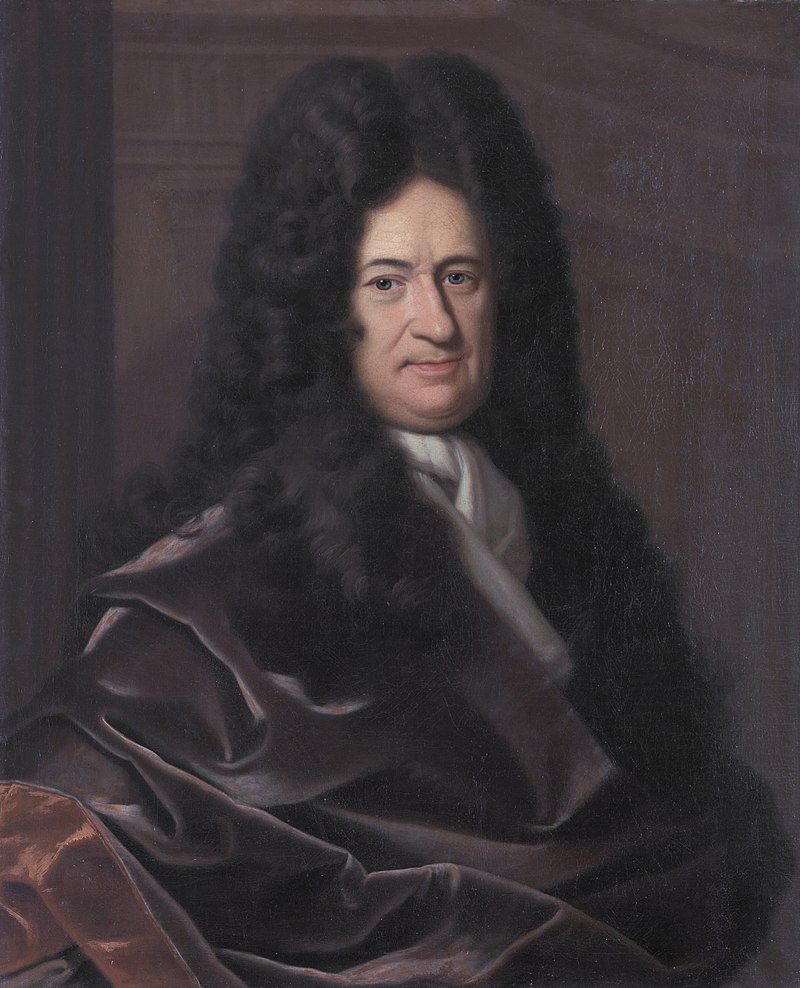
\includegraphics[width=6cm, height=7cm]{Figura_de_Leibniz.jpg}
		\begin{center}
			\textbf{Gottfried Wilhelm von Leibniz (1646-1716)}
		\end{center}
	\end{figure}
	
	\newpage
	\noindent
	Los primeros intentos orientados en la búsqueda de métodos generales para integrar las ecuaciones diferenciales iniciaron cuando Newton (1642-1727), contrastó las ecuaciones diferenciales de
	primer orden en tres clases, $dy/dx=f(x)$; $dy/dx=f(x ,y)$ y $x\partial u/\partial x + y\partial u/\partial y=u$.
	Las dos primeras clases tienen solamente las derivadas ordinarias de una o más variables dependientes, con respecto a una sola variable independiente (ordinarias). La última clase tiene derivadas parciales de una variable dependiente, y actualmente se conocen como ecuaciones diferenciales parciales.
	
	\begin{figure}[h]
		\centering
		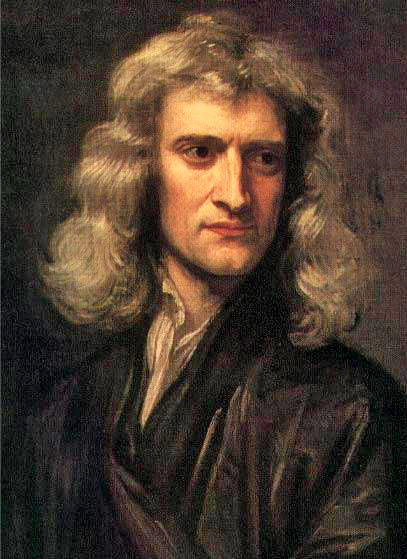
\includegraphics[width=6cm, height=7cm]{Figura_de_Newton.jpg}
		\begin{center}
			\textbf{Isaac Newton (1642-1727)}
		\end{center}
	\end{figure}
	
	\medskip
	\noindent
	La búsqueda de fluxiones le otorgó a Newton una gran cantidad de cuadraturas, y con el tiempo notó la necesidad de agregar en sus trabajos, una constante aditiva. Luego sucedió que la operación de inversión, incluso de ecuaciones sencillas como $Mx'+Ny'=0$, obtenidas en el cálculo de las fluxiones, no siempre podía realizarse y no se obtenía la función original. Newton observó esto cuando $M=M(x,y)$ y $N= N(x,y)$ eran funciones racionales enteras.
	
	\medskip
	\noindent
	Cuando el método directo no era exitoso, Newton recurría al desarrollo de las funciones en series de potencias como herramienta universal
	de la teoría de las fluxiones. La ecuación dada la soluciona, por ejemplo, respecto a $y'/x'$ (o tomando $x=1$) respecto a $y$, y desarrolla en series de potencias la función del miembro derecho, ahora esta serie la integra término a término. Dicho método lo dio a conocer en un anagrama (históricamente, el segundo más importante en su correspondencia con Leibniz, vía Old enburg) y dice lo siguiente: \textit{\textquotedblleft El primer método consiste en la extracción de una cantidad fluente de la ecuación que contiene su fluxión, el segundo en cambio consiste en la mera sustitución de una serie en lugar de una cantidad incógnita cualquiera, de la cual pueden deducirse fácilmente las otras, y en comparación de los términos homólogos de la ecuación resultante para obtener los términos de la serie supuesta\textquotedblright}.
	
	\medskip
	\noindent
	Newton observó que la ecuación tenía un número infinito de soluciones particulares, sin embargo, solo hasta mediados del siglo XVIII se pudo asimilar el significado completo
	de esta observación, en otras palabras, que la solución general de una ecuación de primer orden depende de una constante arbitraria.
	
	\medskip
	\noindent
	Solamente en algunos casos específicos puede una ecuación diferencial ser integrable en una forma finita, esto quiere decir que su solución se puede expresar mediante un número finito de funciones conocidas. El caso general, depende de soluciones escritas como series infinitas, y sus coeficientes se determinan mediante fórmulas de recurrencia.
	
	\medskip
	\noindent
	En 1682, Leibniz se convirtió en un colaborador \textit{habitué} de la nueva revista de Leipzig, Acta Eruditorum, en ella publicó seis trabajos sobre cálculo diferencial en 1684, que marcaron historia. Dos años después (en 1686) publicó un artículo que contienía las nociones básicas del cálculo integral.
	
	\medskip
	\noindent
	Para los creadores del Calculus, la integración de las ecuaciones diferenciales, era un problema que en sus inicios, estaba contenido en un problema más general: el problema inverso del análisis infinitesimal. Como debería esperarse, al principio la atención estaba enfocada en las ecuaciones de primer orden. Se buscaba que las soluciones tuvieran una forma de funciones algebraicas o trascendentes elementales, empleando métodos más o menos exitosamente elegidos. Los pioneros del análisis y sus discípulos redujeron este problema a la operación de búsqueda de funciones primitivas, y para ello, tendían a separar las variables en cada ecuación diferencial. Este es el método con el que inician los textos actuales de la teoría de ecuaciones diferenciales, y al parecer fue históricamente el primero.
	
	\medskip
	\noindent
	Es importante señalar que la expresión \textbf{aequatio differentialis}, fue utilizada por primera vez por Leibniz (con un enfoque bastante restringido) en 1676 para denotar una relación entre las diferenciales $dx$ y $dy$ y dos variables $x$ e $y$; este concepto fue conservado hasta los tiempos de Euler (en los años 1768-1770). También es importante recordar (como ya se dijo anteriormente), que las Ecuaciones Diferenciales Ordinarias aparecieron prácticamente con el surgimiento del Calculus. En la famosa polémica Newton-Leibniz hay un singular momento y tiene que ver con que Newton comunica (a través de Oldenburg) a Leibniz el siguiente anagrama:
	\[
	6a \ \ ce \ \ d \ \ ae\ \ 13e \ \ ff \ \ 7i \ \ el \ \ 9n \ \ 4o \ \ 4q \ \ rr \ \ 4s \ \ 9t \ \ 12v \ \ x
	\]
	que en latín significa \textit{\textquotedblleft Data aequetione quotcunque fliuentes quantitaes involvente fluxiones invenire et viceversa\textquotedblright}, o bien: \textit{\textquotedblleft Dada una ecuación con cantidades fluentes, determinar las fluxiones y viceversa\textquotedblright}. Arnold menciona que este fue el descubrimiento fundamental de Newton que consideró necesario mantener en secreto, y en lenguaje matemático contemporáneo significa: \textit{\textquotedblleft Es útil resolver ecuaciones diferenciales\textquotedblright}.
	
	\medskip
	\noindent
	Antes de abandonar el momento histórico de Newton-Leibniz, resaltemos algunos de los aspectos más importantes:
	\begin{itemize}
		\item[1.] En este periodo de tiempo, los problemas continuaban tratándose con ideas geométrico euclidianas. Leibniz y Newton, elaboran sus trabajos matemáticos en términos de entes geométricos con los
		que representan propiedades y conceptos. Esto debido a lo restringido que estaba el concepto de función en el siglo XVII. La noción de función estaba aún asociada a la idea de curva geométrica. Por ello, el concepto de tangente era el euclidiano. Con Leibniz se tenía un elemento diferente pero era ambiguo, y consistía en entender la recta tangente como aquella que une dos puntos infinitamente próximos. De cualquier forma, la idea que se tenía de recta tangente era totalmente intuitiva.
		\item[2.] Tanto el cálculo de Newton como el de Leibniz, trataban de cantidades variables. Con Leibniz una sucesión de valores infinitamente próximos; y con Newton cantidades que variaban respecto del tiempo. El primero entiende el continuo geométrico como aquel que está formado por segmentos infinitesimales. En el segundo hay un enfoque intuitivo de movimiento continuo que se aproxima al concepto
		de límite. Para Newton lo indefinidamente pequeño debía referirse en términos de últimas razones.
	\end{itemize}
	
	\medskip
	\noindent
	Durante la última década del siglo XVII los hermanos Bernoulli (James y Johan), incluyeron algunos términos tales como \textquotedblleft integrarüna ecuación diferencial\textquotedblright, y también introdujeron
	el método de \textquotedblleft separación de variables\textquotedblright (\textbf{separatio indeterrninatarurn}) de una ecuación diferencial, así inicia una época que estuvo influenciada por los trabajos de esta familia.
	
	\medskip
	\noindent
	James Bernoulli (1654-1705) envió en 1687 una carta a Leibniz, en la que le pidió una iniciación en los misterios del nuevo análisis. Dado que Leibniz estaba de viaje en el exterior, dicha carta quedó sin respuesta hasta 1690. No obstante, James y su hermano Johan Bernoulli (1667-1748) \textquotedblleft descifraron\textquotedblright\ los misterios sin ayuda. Luego inició una extensa comunicación por cartas con Leibniz. En dichas cartas se dieron a conocer muchas innovaciones y anticipaciones de los procedimientos más relevantes. En 1692 James dio a conocer el método para integrar la ecuación diferencial homogénea de primer orden, y poco tiempo después llevó a cuadraturas el problema de integrar una ecuación lineal de primer orden. Los mayores y legítimos descubrimientos de, prácticamente todos los métodos elementales conocidos para resolver las ecuaciones diferenciales de primer orden, se obtuvieron con la dinastía de los Bernoulli.
	
	\medskip
	\noindent
	Los Bernoulli fueron una familia suiza de eruditos, y sus aportes al desarrollo de las ecuaciones diferenciales, se dieron en los siglos XVII y XVIII (ocho representantes de tres generaciones de esta familia, se distinguieron en el campo
	de las Matemáticas). El progenitor de esta famosa familia de matemáticos fue Nikolaus Bernoulli (1623-1708). James I, Johan I, y Daniel son los integrantes más conocidos de la familia Bernoulli, gracias a sus abundantes contribuciones en el nuevo campo de las ecuaciones diferenciales.
	
	\chapter{Clasificación de las ecuaciones diferenciales}
	
	\section{Tipo, orden y linealidad de una ecuación diferencial}
	\noindent
	Las ecuaciones diferenciales se clasifican según su tipo, orden y linealidad.
	
	\medskip
	\noindent
	\textbf{Clasificación por tipo.} Si una ecuación contiene solo derivadas ordinarias de una o más variables dependientes con respecto a una sola variable independiente se dice que es una \textbf{ecuación diferencial ordinaria (EDO)}. Por ejemplo, las siguientes ecuaciones son ecuaciones diferenciales ordinarias:
	\[
	\frac{dy}{dx} + 10y = x^2, \hspace{0.5cm} \frac{d^2y}{dx^2} - \frac{dy}{dx} + 3y = 0, \hspace{0.5cm} \frac{dy}{dt} + \frac{dx}{dt} = 3x-y
	\]
	
	\noindent
	Una ecuación con derivadas parciales de una o más variables dependientes de dos o más variables independientes se llama \textbf{ecuación diferencial parcial (EDP)}. Por ejemplo, las siguientes ecuaciones son ecuaciones diferenciales parciales:
	\[
	 \frac{\partial^2U}{\partial x^2} + \frac{\partial^2U}{\partial y^2} = 0, \hspace{0.5cm} \frac{\partial^2U}{\partial y^2} =  \frac{\partial^2U}{\partial x^2} + 3\frac{\partial U}{\partial x} , \hspace{0.5cm} \frac{\partial U}{\partial x} = \frac{\partial V}{\partial t}
	\]
	
	\noindent
	\textbf{Clasificación según el orden.} El orden de una ecuación diferencial (EDO o EDP) es el orden de la derivada mayor en la ecuación. Por ejemplo, la siguiente es una EDO de orden 2:
	\[
	  \frac{d^2y}{d x^2} - 3\left(\frac{d y}{d x}\right)^4 - 10y = x^2 + 1.
	\]
	
	\noindent
	\textbf{Clasificación por linealidad.} Una ecuación diferencial ordinaria de orden $n$ se dice que es lineal, si es de la forma:
	\[
	 a_n(x)\frac{d^ny}{d x^n} + a_{n-1}(x)\frac{d^{n-1}y}{d x^{n-1}} + \cdots + a_1(x)\frac{dy}{d x} + a_0(x)y = g(x)
	\]
	y satisface las siguientes condiciones:
	\begin{itemize}
		\item La variable dependiente $y$ y todas sus derivadas $y'$, $y''$, $\ldots \ $, $y^n$ son de primer grado, es decir, la potencia de cada término en que interviene $y$ es 1.
		\item $a_0(x)$, $a_1(x)$, $\ldots \ $, $a_n(x)$ y $g(x)$ son funciones que dependen solo de la variable $x$, siendo $a_n(x)\neq0$.
	\end{itemize}
    
    \medskip
    \noindent
    Por ejemplo, la siguiente EDO de orden 2 es lineal: 
    	\[
    (x^2+1)\frac{d^2y}{d x^2} + x\frac{dy}{d x} - 2y = e^x.
    \]
    
    \section{Ejercicio resuelto}
    \noindent
    Para terminar, vamos a resolver un ejercicio sobre ecuaciones diferenciales.
    
    \medskip
    \noindent
    \textbf{Ejercicio:} la pendiente de una familia de curvas en cualquier punto $(x,y)$ del plano $xy$ está dada por $f(x)=4-2x$.
    \begin{itemize}
    	\item[a)] Establezca la ecuación diferencial de la familia.
    	\item[b)] Determine el elemento de la familia que pasa por el punto $(0,1)$.	
    \end{itemize}
    
    \medskip
    \noindent
    \textbf{Solución.} 
    \begin{itemize}
    	\item[a)] La pendiente $m$ de acuerdo al enunciado es:
                    \[
                      m = \frac{dy}{dx} = 4 - 2x \hspace{0.5cm} \longrightarrow \hspace{0.5cm} \text{EDO separable, de primer grado, lineal}
                    \]
                  que representa la ecuación diferencial de la familia.
        \item[b)] Para resolver este inciso se requiere la solución general de la ecuación diferencial, es decir, la función $y(x)$. Entonces al integrar:
        \begin{align*}
        	& dy = (4-2x)dx \\
        	\\& \int dy = \int (4-2x)dx \\
        	\\& y(x) = 4x - x^2 + C \hspace{0.5cm} \longrightarrow \hspace{0.5cm} \text{Solución general a la EDO}.
        \end{align*}
    Para la condición $x=0$, $y=1$ al sustituir en la solución general se tiene: $C=1$.
    Finalmente, sustituyendo este valor de $C$ en la solución general, se obtiene:
    \[
      y(x) = 4x - x^2 + 1  \hspace{0.3cm} \text{que representa la solución particular de la EDO}.
    \]
    
    \newpage
    
    A continuación se presenta el código en Matlab en la versión R2015b, que resuelve el anterior ejercicio de la ecuación diferencial ordinaria, de variable separable, de primer orden y lineal, con condición inicial. \\
            
    \begin{lstlisting}[frame=single]
	%%%%%%%%%%%%%%%%%%%%% Matlab R2015b %%%%%%%%%%%%%%%%%%%%%
	%%%% Scrip que resuelve una EDO separable, lineal, de primer 
	%%%% grado por medio del comando dsolve(), con condicion inicial
	
	% dsolve() da la solucion particular de la EDO
	solP = dsolve( 'Dy = 4-2*x', 'y(0) = 1','x' )
	
	% Genero un vector x con valores desde -2 hasta 5, de 500 elementos
	x = linspace(-2, 5, 500);
	% Evaluo la solucion particular de la EDO con los valores del vector x
	y = eval( vectorize( solP ) );
	
	%%%% Graficando la solucion particular y condicion inicial
	% Dandole un nombre a la figura o ventana
	figure('Name' , 'Angie Melissa Bravo Gonzalez') 
	plot(x, y, 'red', 0, 1, '-s')% Graficando x, y, y(0)=1
	% Dandole un titulo a la grafica
	title('Solucion particular y(x) = 1 - x(x - 4), satisface y(0) = 1')
	xlabel('x') % Etiquetando el eje x
	ylabel('y(x)') % Etiquetando el eje y
	legend('y(x) = 1 - x(x - 4)','y(0) = 1') % Convencion de las funciones
	axis([-1 5 -1 5.3]) % Definiendo el area del plano xy a mostrar
	
	%%%% Mostrando resultados por consola con fprintf()
	fprintf('\nAplicacion Que Resuelve La EDO De Variable Separable:')
	fprintf('\n\tdy/dx = 4 - 2x  con y(x=0) = 1')
	fprintf('\n\nCuya solucion, encontrada a mano con la condicion inicial es:')
	fprintf('\n\ty(x) = 4x - x^2 + 1\n\n')
	
	fprintf('Ahora, la EDO a solucionar con el comando dsolve():\n');
	fprintf('\tdy/dx = 4 - 2x\n');
	fprintf('Con condicion inicial:\n');
	fprintf('\ty(0) = 1\n\n');
	
	fprintf('Es (Solucion Particular de la EDO): \n\ty(x) = ');
	% disp() para mostrar por consola una expresion con variables simbolicas.
	disp(solP); 
	
	fprintf('Ahora bien, si comparamos las 2 soluciones, a mano y por Matlab, son las mismas,\n');
	fprintf('solo hay que expandir la solucion dada por Matlab para ver la igualdad de ellas.\n\n');
	\end{lstlisting}
       \newpage
       Ahora, se presenta la gráfica de la solución particular de la ecuación diferencial $y(x)=4x-x_{2}+1$ y su condición inicia $y(0)=1$:\\
       
       \begin{tikzpicture}
       	\begin{axis}[ title=Gráfica de la solución particular y condición inicial, width=10cm, height=6cm, xmin=-1, xmax=5, ymin=-2, ymax=6, xlabel={x}, ylabel={y(x)}, xmajorgrids=true, ymajorgrids=true ]
       		%Below the red parabola is defined
       		\addplot [ domain=-1:5, samples=200, color=red ]{4*x - x^2 + 1};       		\addlegendentry{\(y(x)=4x - x^2 + 1\)}
       		       		
       		\addplot[ color=blue, mark=square ]coordinates{ (0,1) };\addlegendentry{\(y(0)=1\)}
       		
       	\end{axis}
       \end{tikzpicture}
       
    \end{itemize}
    
    \chapter*{Conclusiones}
    \begin{itemize}
    	\item A finales del siglo XVII e inicios del siglo XVIII, los matemáticos sostuvieron encarnizadas rivalidades matemáticas al tratar de resolver problemas relacionados con ecuaciones diferenciales, esto generó un ambiente altamente competitivo en la comunidad matemática de este tiempo.
    	\item A ningún matemático que haya trabajado en ecuaciones diferenciales durante los siglos XVII y XVIII, se le puede atribuir el desarrollo completo de un resultado relacionado con ecuaciones diferenciales.
    	\item 	Las ecuaciones diferenciales se clasifican según su tipo, orden y linealidad. Esta clasificación permite que la teoría sobre ecuaciones diferenciales tenga una jerarquía dentro de las matemáticas, ubicándola como una de las teorías más importantes y aplicativas de las matemáticas.
    \end{itemize}
    
	
	\newpage
	\noindent
	\begin{thebibliography}{55}
		
		\bibitem{} Bernoulli, J. (1955). Der Briefwechsel von Johann Bernoulli. Birkhauser Verlag, pp. 97-98.
		\smallskip
		\bibitem{} Cullen, M., Zill, D. (2009). Ecuaciones diferenciales con problemas con valores en la frontera, Séptima edición.
		ISBN-13: 978-607-481-314-2, ISBN-10: 607-481-314-0.
		\smallskip
		\bibitem{} Kline, M. (1992). El pensamiento matematico de la antigüedad a nuestros días Vols 1, 2 y 3. Alianza Editorial S.A. Madrid.
		\smallskip
		\bibitem{} Leibniz-Newton (1977). El Cálculo Infinitesimal origen-polémica, Editorial Universitaria de Buenos Aires, p. 29.
		\smallskip
		\bibitem{} Martínez, M. (1984). Del cálculo a la teoría de conjuntos, 1630-1910 Una introducción histórica Compilación de I. Grattan-Guiness. Alianza Editorial, S.A. Madrid.
		\smallskip
		\bibitem{} Nápoles, J. E. (2008). De Leibniz a D' Alembert: diez problemas que marcaron un siglo. Boletín de Matemáticas Nueva Serie, Volumen XV No. 2 (2008), pp. 130-161.
		\smallskip
		\bibitem{} Recalde, L. C., Henao S. M. (2018). Los obstáculos epistemológicos en el desarrollo histórico de las ecuaciones diferenciales ordinarias. Revista EIA, ISSN 1794-1237 / Año XV / Volumen 15 / Edición N.29 / Enero-Junio 2018 / pp. 59-70 Publicación semestral de carácter técnico-científico / Universidad EIA, Envigado (Colombia).
		\smallskip
		\bibitem{} Struik, D. J. (1969). A Source Book in Mathematics, 1200-1800. Cambridge, Mass., Harvard University Press.
		\smallskip
	\end{thebibliography}		
\end{document}